\section{Wat zijn zelflerende computersystemen?}

\subsection{Inleiding}
Elk jaar boekt de mens grootschalige vorderingen op het gebied van computers, zowel hardware als software. Iets waar wij echter nog niet in geslaagd zijn te maken is een ware \textbf{ Artificial Intelligence}, al lukt het steeds beter de schijn van denken te creëren. Voorbeelden zijn de \textit{persoonlijke assistenten} die inmiddels in elke smartphone geïntegreerd zijn. \textit{Siri}, \textit{Google Now} en \textit{Cortana} maken gebruik van spraakherkenning om de gebruiker de gevraagde informatie te tonen, maar denken zoals mensen doen ze hierbij niet. Hoe een computersysteem toch beter kan worden in het imiteren van menselijk gedrag en van zijn eigen fouten kan leren onderzoeken we in deze deelvraag.


\subsection{Verschillende algoritmes}
Computers hebben geen dus bewustzijn. Om deze reden kunnen ze niet zelf bepalen iets te doen. Waar computers wel in uitblinken, is het uitvoeren van taken die ze zijn opgelegd. Vaak komen deze taken in de vorm van code. Via code kan je computers opdrachten geven, bijvoorbeeld laat een scherm zien. De boodschap valt echter niet op deze manier over te brengen, afhankelijk van de taal waarin je programmeert zijn er vaste commando's waar de computer op zal reageren.
Naarmate de opdracht die je een computer wil laten uitvoeren complexer wordt, zal ook het gebruik in deze commando's een verandering zien. Hier komen algoritmes in het spel. Een algoritme is een soort stappenplan voor de computer, waarin een complexere handeling in duidelijke opdrachten weergegeven wordt. De volgende definitie geeft een betekenis in de meest algemene zin: een algoritme is een eindige reeks instructies om vanaf een beginpunt een bepaald doel te bereiken.\cite{WoordenOrg}

Een toegankelijke vergelijking is koken. Er is een \textbf{input} van voedsel waar uiteindelijk een gerecht uit moet komen, de \textbf{output}. Voor het tot stand komen van dit gerecht gebruik je misschien een recept. Dit recept is als het ware het algoritme.
Uit de gegeven definitie is af te leiden dat het aantal mogelijke algoritmes ontzettend groot is. Niet alleen is het een ruim begrip, ook kan het desbetreffende doel waarschijnlijk op meerdere manieren bereikt worden. In deze verschillende methodes kan de een echter beter zijn dan de andere, bijvoorbeeld door effici\"enter te zijn.

Uiteraard zijn er ook vele algoritmes die gebruik maken van toepassingen, zoals een \textbf{queue} en een \textbf{stack}, die betrekking hebben tot ons onderwerp. Enkele hiervan zullen hier beschreven worden:

\subsection{Breadth-first search (BFS)}
Dit algoritme, bedacht in de jaren vijftig van de vorige eeuw door E.F. Moore[b], een Amerikaans professor in de wiskunde en computer sciences en een voortrekker in kunstmatig leven, is een zoekalgoritme voor datasets in de vorm van grafieken of 'boom'-structuren. In deze dataset wordt een \textbf{node} als oorsprong benoemd, de \textbf{root}. Ook wordt een bepaalde uitkomst als doel gesteld. Vervolgens krijgt elke node drie waardes aangewezen:
\begin{itemize}
\item De afstand van de huidige node naar de root. Dit is het aantal stappen dat gezet moet worden om bij de root te komen. \blindtext
\item De node die v\'{o}\'{o}r de huidige node kwam, de \textbf{predecessor}. Anders gezegd: bij welke node je uitkomt als je een enkele stap terug zet. \blindtext
\item Een \textbf{state}. De state houdt bij of een node al gecontroleerd is. \blindtext
\end{itemize}

Bij Breadth-first search wordt gebruik gemaakt van een queue. Dit is een lijst waar nodes aan toegevoegd en uitgehaald kunnen worden. Net zoals een daadwerkelijke wachtrij wordt het `als eerste erin, als eerste eruit' principe toegepast.

\begin{enumerate}
\item Maak een lege lijst S voor bezochte nodes.\blindtext
\item Maak een lege lijst Q met de queue.\blindtext
\item Benoem één node als root en voeg deze toe aan S.\blindtext
\item Voeg de root toe aan Q.\blindtext
\item Terwijl Q niet leeg is:
	\begin{enumerate}
	\item Haal de voorste node uit de queue. Dit is de 'current' node.\blindtext
	\item Als current het doel is:\blindtext
		\begin{enumerate}
		\item Return current.\blindtext
		\end{enumerate}
	\item Voor elke node die grenst aan* current:\blindtext
		\begin{enumerate}
		\item Als deze node nog niet bezocht is en dus niet in S zit:\blindtext
			\begin{enumerate}
			\item Voeg de node toe aan S.\blindtext
			\item Zeg dat de predecessor van de node de current node is.\blindtext
			\item Haal de node uit de queue.\blindtext
			\end{enumerate}
		\end{enumerate}
	\end{enumerate}
\blindtext
\end{enumerate}

\textit{*Aangrenzend zijn betekent hier `in directe verbinding staan met'.}

\begin{figure}[h]
  \centering
    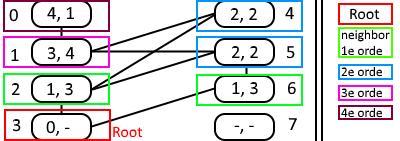
\includegraphics[width=\textwidth]{datasetBFS3.png}
  \caption{Schematische weergave van een willekeurige dataset. De volgorde waarin de nodes bezocht worden is 3 – 2 – 6 – 4 – 5 – 1 – 0.}
  \label{fig:datasetBFS3}
\end{figure}

Hierboven is een voorbeeld van een simpele dataset weergegeven, genummerd van 0 tot en met 7. Node 3 is de root en 0 het doel. Voor het gemak staan in elke node twee getallen: de afstand tot 3 en het nummer van de predecessor. Met kleuren zijn aangegeven in welke volgorde de nodes bezocht worden.
3 is de root. 3 wordt toegevoegd aan de lijsten Q en S. Hierdoor is de queue niet leeg. 3 wordt weer uit de queue gehaald en één voor één worden de aangrenzende nodes bekeken. Hierbij worden ze toegevoegd aan de stack. Omdat zowel 2 als 6 het niet het doel is, herhaald het algoritme zich. Nu wordt 2 gecheckt. Het doel is niet gevonden. Daarna 6, ook zonder succes. (Let hierbij op dat node 5 niet nogmaals gecheckt wordt, dit is namelijk als bij node 2 gedaan en is dus al aanwezig in lijst S) Intussen zij 4 en 5 toegevoegd aan de queue, ze zijn immers verbonden met 2. Ook hier wordt het proces herhaald, node 1 zit nu in de queue. Uiteindelijk wordt node 1 gecheckt en wordt het doel, node 0, gevonden.

Met BFS kan je de weg van de root naar het doel achterhalen. Dit is nuttig als je bijvoorbeeld een wegennetwerk hebt en wil weten wat de kortste weg van de ene naar de andere stad is.


\subsection{Depth-first search (DFS)}
Evenals breadth-first search is depth-first search een algoritme voor het doorlopen van datasets in grafieken of trees. DFS verschilt echter op twee manieren van BFS:

\begin{itemize}
\item Depth-first search gebruikt een stack in plaats van een queue. Waar nodes in een BFS systeem in een wachtrij werden geplaats met een `Als eerst erin, als eerst eruit' principe, handhaaft een DFS systeem een wachtrij meer vergelijkbaar met een stapel papieren. Telkens pak je het bovenste element van de stapel om mee te werken, maar als je iets in de wachtrij stopt, komt dit ook weer bovenop de stapel te liggen. De meest recente toevoeging zal dus als eerste weer eruit gehaald worden.\blindtext
\item Breadth-first search begon bij een root. Vervolgens werd gekeken naar alle neighbors. Als de gewenste uitkomst niet tussen deze neighbors zit, worden de neighbors van deze neighbors gecontroleerd. Dit proces herhaalt zich totdat het doel gevonden is.
Depth-first search begint ook bij een root, maar kijkt direct naar een weg tot een node bereikt is die geen neighbors meer heeft. Als het doel dan niet bereikt is wordt een andere weg geprobeerd. Hiervoor wordt gebruik gemaakt van \textbf{recursive backtracking}.
\blindtext
\end{itemize}

\begin{figure}[h]
  \centering
    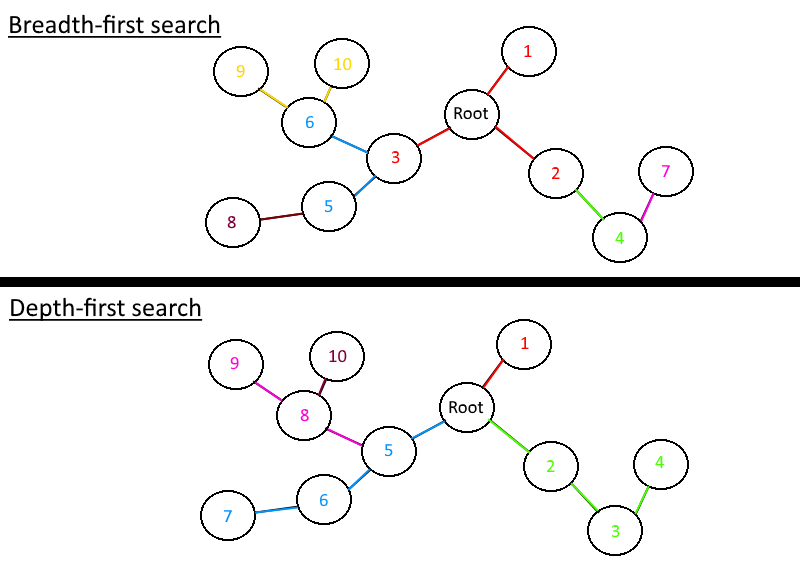
\includegraphics[width=\textwidth]{verschil-BFS-DFS.png}
  \caption{Schematische weergave van een willekeurige dataset.}
  \label{fig:verschil-BFS-DFS}
\end{figure}

In figuur ****  is de werking van BFS en DFS weergegeven. Het getal in elke node geeft aan als hoeveelste het bereikt wordt. De kleuren representeren de gebieden die het algoritme per stap doorloopt.

Ook bij DFS hebben de nodes een state: bezocht of niet bezocht.
Ten eerste wordt de root gekozen en wordt deze als bezocht opgeslagen. Zoals te zien wordt er vanaf de root één (willekeurige) neighbor gekozen om te onderzoeken. Elke bezochte neighbor wordt als bezocht genoteerd. De root wordt in de stack geplaats. Als de gekozen neighbor niet het doel is, wordt de meest recentelijk toegevoegde node, de root, gehaald, de eerst bezochte had immers geen aanliggende nodes om te onderzoeken. Deze tweede neighbor, cirkel 2 in de figuur, heeft wel een neighbor. Deze wordt gecontroleerd, evenals diens neighbors. Telkens wordt de huidige node toegevoegd aan de stack.\\
Als het programma de laatste in een reeks nodes bereikt heeft, wordt de bovenste node uit de stack gepakt en gekeken of daar nog niet bezochte nodes aan grenzen. Dit wordt backtracking genoemd.
Dit proces wordt herhaald totdat het doel gevonden is of totdat alle nodes geweest zijn.

Als vuistregel kan het volgende gehanteerd worden: depth-first search wordt gebruikt als je weet dat er maar één uitkomst is, breadth-first search als je de kortste weg wil weten.
\subsection{Voorbeelden algoritmes}
Algoritmes hebben meestal vele toepassingen. Hier zijn enkele voorbeelden van de eerder genoemde algoritmes.
\subsubsection{Breadth-first search}
\begin{figure}[h]
  \centering
    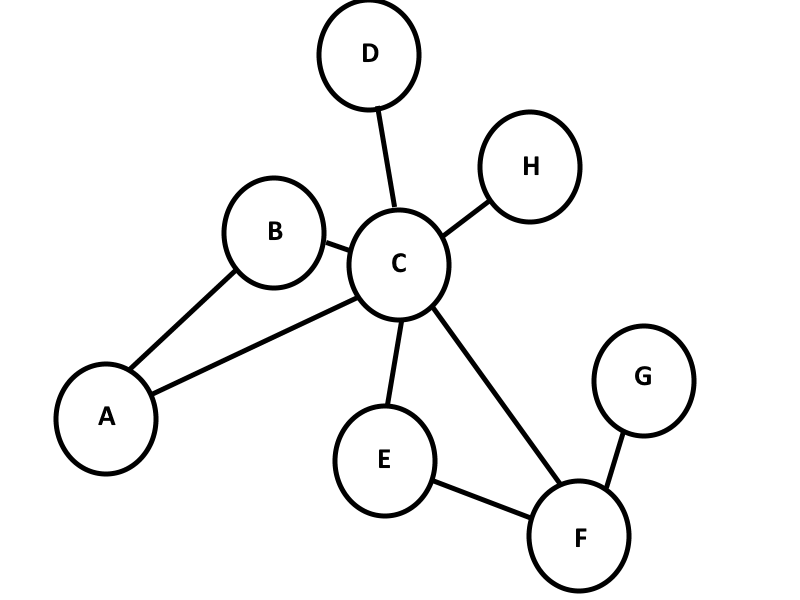
\includegraphics[width=\textwidth]{datasetBFS2.png}
  \caption{Schematische weergave van een willekeurige dataset.}
  \label{fig:datasetBFS2}
\end{figure}

In figuur **** is een dataset te zien, bijvoorbeeld een telefoonboom. Elke cirkel representeert een persoon. Zo kan persoon A de personen B en C bellen, maar A bezit geen andere telefoonnummers. Toch zou hij een boodschap naar H kunnen sturen: via C. 
Stel, persoon A wil nu iets tegen F zeggen. In een kleine dataset als deze is makkelijk met het oog te zien dat de snelste manier hiervoor A – C – F is en dat A – B – C – E – F veel langer is. Bij grotere datasets is dit echter al snel moeilijk met zekerheid te zeggen. Hiervoor kan breadth-first search ingezet worden.

\subsubsection{Depth-first search}
\begin{figure}[h]
  \centering
    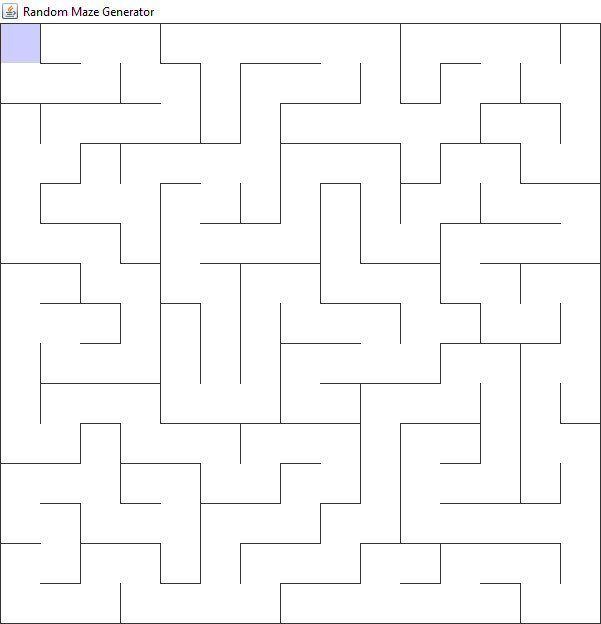
\includegraphics[width=\textwidth]{maze.png}
  \caption{Een voorbeeld van een automatisch gegenereerd doolhof, gebruik makend van DFS.}
  \label{fig:maze}
\end{figure}

Depth-first search kan gebruikt worden voor zowel het maken als oplossen van doolhoven. In figuur **** is een doolhof te zien dat gemaakt is met behulp van DFS. (****programma gemaakt in kader van deze deelvraag****). Het algoritme in de vorm van een stappenplan is als volgt:

\begin{enumerate}
\item Maak de start cel current en markeer deze als bezocht.\blindtext
\item Terwijl er nog niet bezochte cellen aanwezig zijn:
	\begin{enumerate}
	\item Als current neighbors heeft die nog niet bezocht zijn:
		\begin{enumerate}
		\item Kies willekeurig een van de neighbors\blindtext
		\item Voeg current toe aan de stack\blindtext
		\item Verwijder de muur tussen de huidige cel en de gekozen cel\blindtext
		\item Benoem de gekozen cel als current en zet de state op bezocht\blindtext
		\end{enumerate}			
	\blindtext
	\item Anders, als de stack niet leeg is:
		\begin{enumerate}
		\item Haal de laatst toegevoegde cel uit de stack en verwijder deze hieruit\blindtext
		\item Maak deze cel current\blindtext
		\end{enumerate}	
	\blindtext
	\end{enumerate}
\blindtext
\end{enumerate}
\subsection{Zelflerend?}
Breadth-first search en Depth-first search zijn beide algoritmes met vele toepassingen. Toch kunnen beide algoritmes niet als zelflerend worden beschouwd, ze verbeteren hun manier van zoeken namelijk niet. Hoe zit een zelflerend systeem dan wel in elkaar? Hoe kan een algoritme zichzelf verbeteren?

\subsection{Machine learning}
Een zelflerend systeem is een algoritme gebaseerd op machine learning. Machine learning werd door Arthur Samuel, een pionier op dit gebied, gedefinieerd als: 
\textit{A field of study that gives computers the ability to learn without being explicitly programmed.} \cite{ArthurSamuel} 
In tegenstelling tot de eerder genoemde algoritmes is een zelflerend systeem in staat zichzelf te verbeteren. Hierdoor kan het taken uitvoeren waarbij reguliere algoritmes tekort schieten. Welke taken dit betreft, zullen we in de derde deelvraag behandelen. 

\begin{figure}[h]
  \centering
    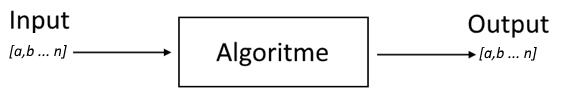
\includegraphics[width=\textwidth]{algorithm1.png}
  \caption{Schematische weergave van een zelflerend systeem}
  \label{fig:algorithm1}
\end{figure}

In figuur \ref{fig:algorithm1}  is een schematische weergave van een zelflerend systeem afgebeeld. Bepaalde input data gaat het systeem in en bepaalde output data komt het systeem uit. De input en output data bestaat uit \'e\'en of meerdere getallen. Als de input simpelweg een reeks getallen betreft, zal dit direct als input gebruikt kunnen worden. In het geval dat de input uit een ander datatype bestaat, zoals een plaatje, zal dit omgezet moeten worden in een reeks getallen voordat het in een zelflerend systeem gebruikt kan worden. Het algoritme zal deze getallen bewerken tot de gewenste output. Deze output wordt eveneens in getallen gegeven. Waar nodig zullen deze getallen dus weer moeten worden omgezet tot het gewenste datatype.

Er zijn veel verschillende algoritmes die gebruikt kunnen worden voor een zelflerend systeem. Elk algoritme heeft voor- en nadelen en is geschikt voor andere doeleinden. Een aantal van deze algoritmes zullen we in de tweede deelvraag behandelen. 

\subsection{Training}

Een zelflerend systeem begint in de meeste gevallen zonder enige kennis van de data. Om de gewenste output te kunnen produceren is het dus nodig om het systeem eerst input data te geven zodat het kan leren. Dit proces wordt het \textbf{trainen} genoemd. Voor het trainen van een zelflerend systeem is training data nodig. Deze data moet gelijk of gelijkwaardig zijn aan de \textit{echte} data. De training data kan in veel verschillende vormen voorkomen en de manier van trainen is afhankelijk van de vorm van de (training) data. In figuur \ref{fig:algorithm2}  is te zien dat het trainen los staat van het algoritme. Dit verschil zullen we in de volgende deelvraag wat duidelijker maken. 
Er zijn drie prominente manieren waarop een zelflerend systeem getraind kan worden: \textbf{supervised}, \textbf{unsupervised} en \textbf{reinforcement learning}.

\begin{figure}[h]
  \centering
    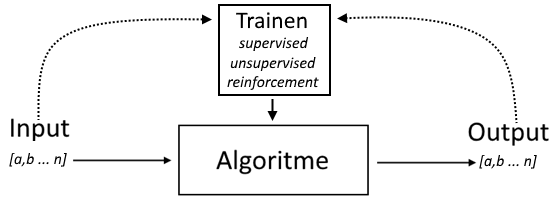
\includegraphics[width=\textwidth]{algorithm2.png}
  \caption{Schematische weergave van een zelflerend systeem}
  \label{fig:algorithm2}
\end{figure}

\subsubsection{Supervised Learning}
In het geval van supervised learning heb je te maken met \textbf{labeled} training data. Anders gezegd: van een bepaalde input is de gewenste output al bekend. Een klassiek voorbeeld van een labeled dataset is een dataset van huisprijzen en huiseigenschappen (zie figuur \ref{fig:LabeledDataset})

\begin{table}[h]
\centering
\begin{tabular}{llll}
\hline
\multicolumn{1}{c}{\multirow{2}{*}{Huisprijs (output)}} & \multicolumn{3}{c}{Huiseigenschappen (input)} \\
\multicolumn{1}{c}{} & \multicolumn{1}{c}{Woonoppervlakte} & \multicolumn{1}{c}{Perceeloppervlakte} & \multicolumn{1}{c}{Aantal Kamers} \\ \hline
€ 519.000 & 124 m² & 311 m² & 4 \\
€ 569.000 & 133 m² & 309 m² & 5 \\
€ 569.500 & 170 m² & 310 m² & 6 \\ \hline
\end{tabular}
\caption{Labeled dataset Bron: http://www.funda.nl/koop/huizen/ }
\label{fig:LabeledDataset}
\end{table}
Bij de training dataset van figuur \ref{fig:LabeledDataset} is de gegeven input de huiseigenschappen en de gewenste output de huisprijs. Het systeem wordt met deze dataset getraind. Hierdoor leert het een output te produceren die steeds dichter bij de gewenste output ligt. Als er een verband bestaat tussen de huiseigenschappen en de huisprijs, wat waarschijnlijk het geval is, zal het zelflerende systeem na genoeg trainen in staat zijn zelf bij nieuwe huiseigenschappen een huisprijs te voorspellen. \cite{MLCourse1}

\subsubsection{Unsupervised Learning}
Unsupervised learning kan gebruikt worden bij een \textbf{unlabeled} dataset ofwel, een dataset waarbij de data niet geclassificeerd is en er geen gewenste output bekend is. Als je een dataset hebt van heel veel niet-geordende foto's is het niet mogelijk om dit te classificeren. Als een deel van de dataset gelabeld wordt, zal met behulp van supervised learning de rest van de dataset geclassificeerd kunnen worden. Dit is echter in veel gevallen niet mogelijk, bijvoorbeeld doordat de dataset enorm groot is of er zodanig veel verschillende groepen bestaan dat het menselijk niet mogelijk is ook maar een deel te labelen. Ook kan het zo zijn dat men niet weet of er een verband aanwezig is. 
Kortom: unsupervised learning wordt gebruikt voor het classificeren van data, zonder dat er groepen vooraf gedefinieerd zijn. Met behulp van deze vorm van training zullen in een grote dataset verbanden kunnen worden ontdekt, die men misschien niet zonder hulp had kunnen achterhalen.\cite{MLCourse2}

\subsubsection{Reinforcement Learning}
Reinforcement learning is een zeer specifieke soort van leren. Er is bij deze vorm van learning geen dataset met input data, maar is er een bepaalde \textbf{context}. In deze context bevindt zich een \textbf{agent}. Een agent is een object dat bepaalde opdrachten kan uitvoeren. De context is een wereld waarin deze agent zich bevindt. Door de agent bij bepaalde acties pluspunten of minpunten te geven kun je bepaald gedrag bevorderen.  

\begin{figure}[h]
  \centering
    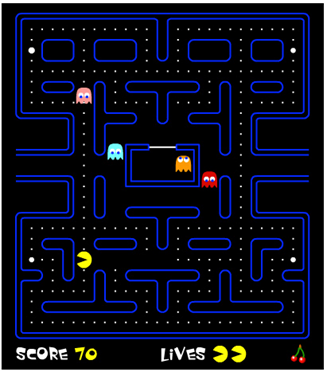
\includegraphics[width=0.5\textwidth]{pacman.png}
  \caption{Pacman}
  \label{fig:Pacman}
\end{figure}

In figuur \ref{fig:Pacman} is het spel Pac-Man te zien. Op dit spel zou reinforcement learning toegepast kunnen worden. De agent is hierbij pacman, dit is namelijk een object dat bepaalde opdrachten kan uitvoeren, zoals: beweeg naar links. De context is hierbij het level, ofwel: de positie van de muren (de blauwe obstakels), de posities van de ghosts (de gekleurde vijanden), de posities van de pac-dots (de kleine stipjes) en de posities van de power-pellets (de grotere stipjes). [4] Het eten van de pac-dots is positief, het geraakt worden door de ghosts is negatief. Door reinforcement learing toe te passen op het spel zal de agent steeds beter worden in het spelen van het spel. 

\subsection{Conclusie}
Zelflerende computersystemen zijn algoritmes gebaseerd op machine learning. Een zelflerend systeem verschilt van reguliere algoritmes zoals breadth-first search en depth-first search doordat ze in staat zijn zichzelf te verbeteren.

\bibliography{references}
\bibliographystyle{plain}